% !TEX TS-program = xelatex
% !TEX encoding = UTF-8 Unicode
% !Mode:: "TeX:UTF-8"

\documentclass{resume}
\usepackage{zh_CN-Adobefonts_external}
\usepackage{graphicx}
\usepackage{multirow}
% Simplified Chinese Support using external fonts (./fonts/zh_CN-Adobe/)

% \usepackage{NotoSansSC_external}
% \usepackage{NotoSerifCJKsc_external}
% \usepackage{zh_CN-Adobefonts_internal}
% Simplified Chinese Support using system fonts
\usepackage{linespacing_fix}
% disable extra space before next section
\usepackage{tabu}

\begin{document}
\pagenumbering{gobble}
% suppress displaying page number
\Large{
  \begin{tabu} to \textwidth { X[1.5,c] X[1.8,c] X[2,c] X[0.8,c]}
    \multicolumn{3}{c}{\bigname{王小明}} &
    \multirow{2}{*}{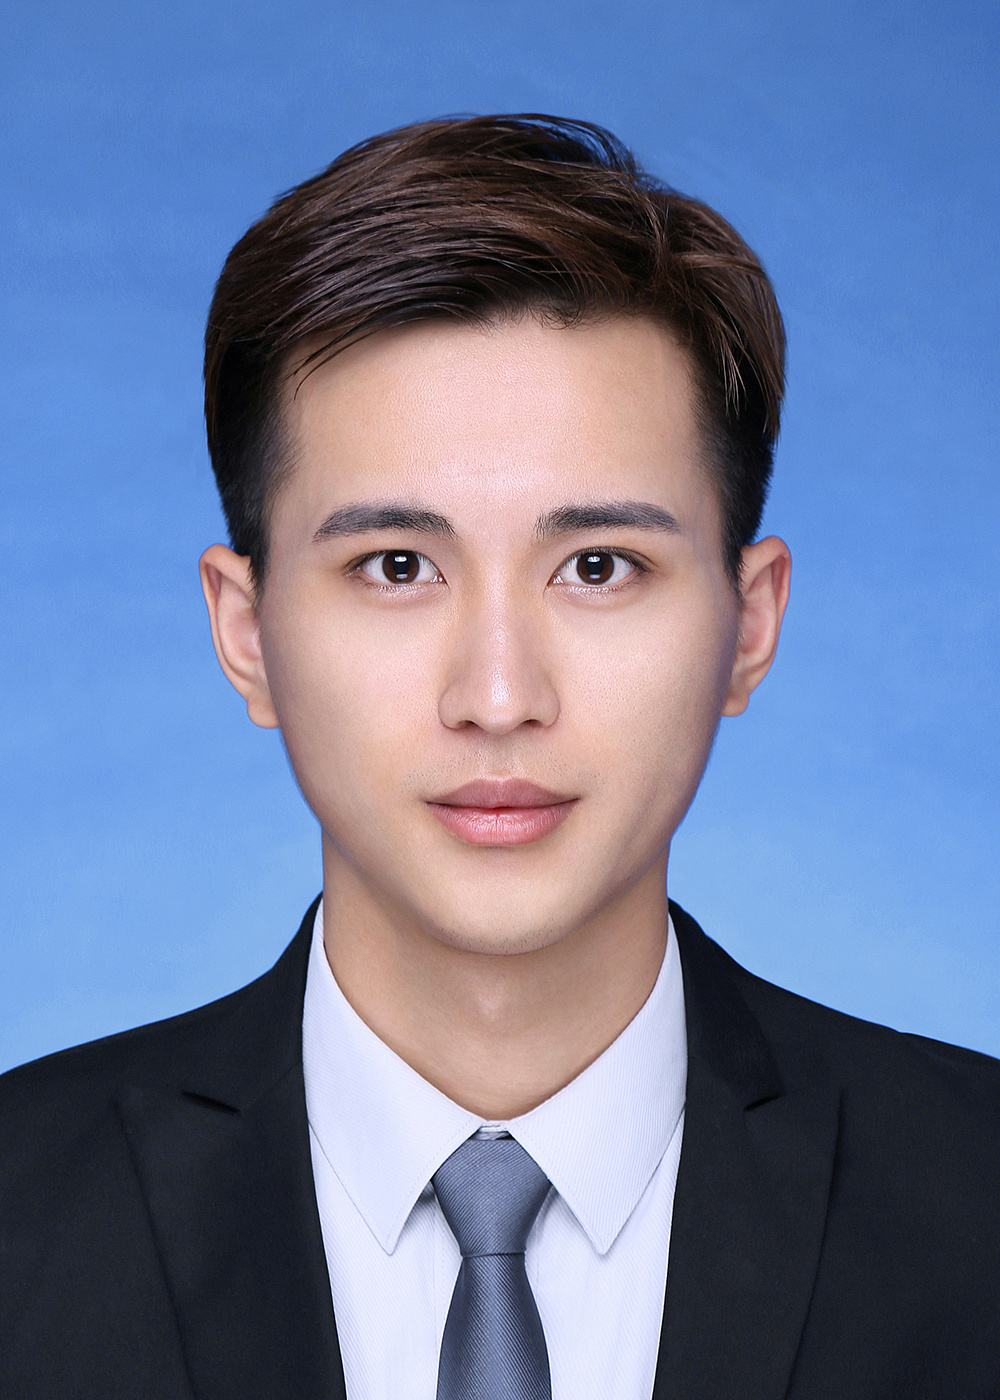
\includegraphics[width=1.8cm]{avatar}}\\
    \multicolumn{3}{c}{\position{机器学习方向实习生\ \ 算法方向实习生\ \ |\ \ 可实习5$\sim$6个月\ \ 随时入职}} \\
    \email{ming@email.com} & \phone{(+86) 188-1234-5678} & \github{https://github.com/ming} & \\
  \end{tabu}
}

\section{教育背景}
\datedsubsection{\textbf{北京科技大学}, 北京}{2016 -- 至今}
\normalsize{\textit{在读硕士研究生}\ 信息与通信工程, 预计2019年1月毕业}
\datedsubsection{\textbf{北京科技大学}, 北京}{2012 -- 2016}
\normalsize{\textit{学士}\ 通信工程,已毕业}

\section{项目经历}
\datedsubsection{\textbf{XXXXXX数据分析}}{实验室合作项目}
\normalsize{首先说明项目的背景来源性质,接着说明自己在项目中参与的工作,最后说明使用了哪些技能。首先说明项目的背景来源性质,接着说明自己在项目中参与的工作,最后说明使用了哪些技能。主要用到的技术包括算法(Python)、分布式计算与存储(Spark+Hadoop)、数据可视化(ECharts.js+PHP)、本地数据库(Oracle)。}


\datedsubsection{\textbf{XXXXXX数据分析}}{实验室合作项目}
\normalsize{首先说明项目的背景来源性质,接着说明自己在项目中参与的工作,最后说明使用了哪些技能。首先说明项目的背景来源性质,接着说明自己在项目中参与的工作,最后说明使用了哪些技能。主要用到的计算包含:常见深度学习算法(PyTorch)、基础矩阵压缩运算(Scipy)、其他辅助功能(Matplotlib、TensorBoard等)。}


\datedsubsection{\textbf{XXXXXX数据分析}}{开源项目,与朋友合作开发}
\normalsize{首先说明项目的背景来源性质,接着说明自己在项目中参与的工作,最后说明使用了哪些技能。首先说明项目的背景来源性质,接着说明自己在项目中参与的工作,最后说明使用了哪些技能。如果能够给出项目主页地址也是最好。\href{项目主页:http://github.com/xxx}{http://github.com/xxx}}

\section{实习经历}
\datedsubsection{\textbf{XXXXXX公司}}{2017-10 $\sim$ 2018-01}
\role{算法实习生}{创业公司,<20人}
\begin{onehalfspacing}
\normalsize{主要负责在线推荐系统的基础搭建和调试、数据清洗工作。其中推荐系统任务是为用户推荐电影。由于公司初创期用户少,且有完善的视频标签分类数据,因此采用的是基于用户的协同过滤与基于内容的协同过滤的加权混合算法,在离线模式中测试良好。项目地址:\href{http://www.baidu.com/}{http://www.baidu.com/}。}
\end{onehalfspacing}

\section{主要技能}
Python(熟练)、JavaScript(熟练)、SQl(熟练)、Linux(掌握)、PHP(基础)、C/C++(入门)\\
机器学习算法(熟练),相关框架(sklearn、numpy、scipy、pandas,掌握)\\
深度学习算法(计算机视觉方面熟练、其他方面基础),相关框架(PyTorch熟练、TensorFlow基础)\\
Spark(基础)、Hadoop+HDFS(入门)

\section{获奖情况}
人民奖学金(2017)、XXXX奖学金(2016)、全国XXXX比赛一等奖(2015)

\section{自我评价}
对新的更好的技术有执着的追求,对机器学习和深度学习领域有浓厚的兴趣。抗压能力强,执行力强。

\end{document}
